\chapter{Plugin Jenkins}

\section{Contexte initial}
!!! ici présentation de Jenkins et des différents plugin avec captures d'écran à l'appuie

\textbf{La solution propos\'{e}e} \hfill \\ \indent
%\subsection{La solution propos\'{e}e}
Le plugin actuel permet de ne prendre en compte que les statuts Jenkins et le claim. La solution serait de pouvoir ajouter un ou plusieurs statut(s) supplémentaire(s). L'ajout de ce nouveau statuts devra se faire de manière générique de sorte que n'importe quel status puissant être ajouté, quelque soit le projet ou le langage utilisé.



\section{étude préalable}
d'abord je me suis renseigné sur Jenkins et ai appris à l'utiliser. Installation, quelques projets de test, installation plugin junit et radiator + appris à les utiliser\\
j'ai passé du temps sur l'étude de junit\\
J'ai regardé comment étendre Jenkins, il me fallait utiliser maven. J'ai donc pris le temps de parfaire mes connaissances sur maven\\
J'ai importé le code du plugin Radiator et l'ai étudié pour comprendre son fonctionnement\\
J'ai importé le code source de Jenkins pour aller chercher les informations qu'il me fallait, la création d'un plugin est très peu documentée\\

A cette période du projet, ma suite de logiciels était la suivante :
\begin{itemize}
	\item l'IDE Eclipse pour développer le plugin, puisque c'est mon IDE de prédilection, open-source et possédant la plus grande communauté. 
	\item Maven m'a servi d'une part à générer l'archétype du plugin mais aussi et surtout il me servait à compiler le code pour obtenir le bon fichier .hpi\footnote{l'extension .hpi est le type reconnu par Jenkins comme étant un plugin}
	\item Jenkins installé sur ma machine en tant que service local configuré de la même manière que le Jenkins utilisé à SAP
	
\end{itemize}

De cette manière mon cycle de développement était le suivant

\begin{enumerate}
	\item Implémentation du code sous Eclipse
	\item Compilation du code grâce à maven et génération du fichier .hpi
	\item Désinstallation du plugin de Jenkins + redémarrage
	\item Installation du nouveau plugin sur Jenkins + redémarrage
	\item Test du plugin
\end{enumerate}
Les inconvénients de cette configuration sont nombreux et très dérangeant pour le cycle de développement.

!!! ici description de certains problèmes !!! \\
un code compile puis ne compile plus sans aucune modif\\
Problème de version de jenkins\\
Très difficile de comprendre comment se passe l'exécution du plugin lorsqu'il est en prod puisqu'impossible de debbugger. à part d'utiliser maven le debugger de maven en remote\\


après meeting avec Pascal DUCAULE qui avais déjà développé un plugin, j'ai changé d'IDE pour utiliser NetBeans qui offre la possibilité de run et de debug le plugin directement depuis l'IDE (NetBeans encapsule une instance de Jenkins). \\
Il suffit d'installer NetBeans, le plugin Jenkins et de configurer les ports utilisés (puisque le 8080 est déjà utilisé par le Jenkins local sur ma machine)



\subsection{Description de la base d'un plugin Jenkins}
\subsubsection{Création du plugin Jenkins}


figure \ref{figure:hpiCreate} page \pageref{figure:hpiCreate}

\begin{figure}[!h]% h || ht || .... cf 
  \centering
      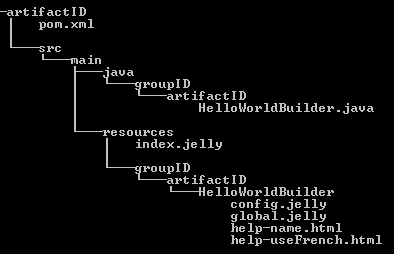
\includegraphics{images/hpiCreate.png}
  \caption{Architecture d'un plugin Jenkins généré par maven}
	\label{figure:hpiCreate}
\end{figure}

\subsubsection{Architecture du plugin et fichiers essentiels}



\section{Investigation et r\'{e}solution}


